\begin{figure}[H]
\centering
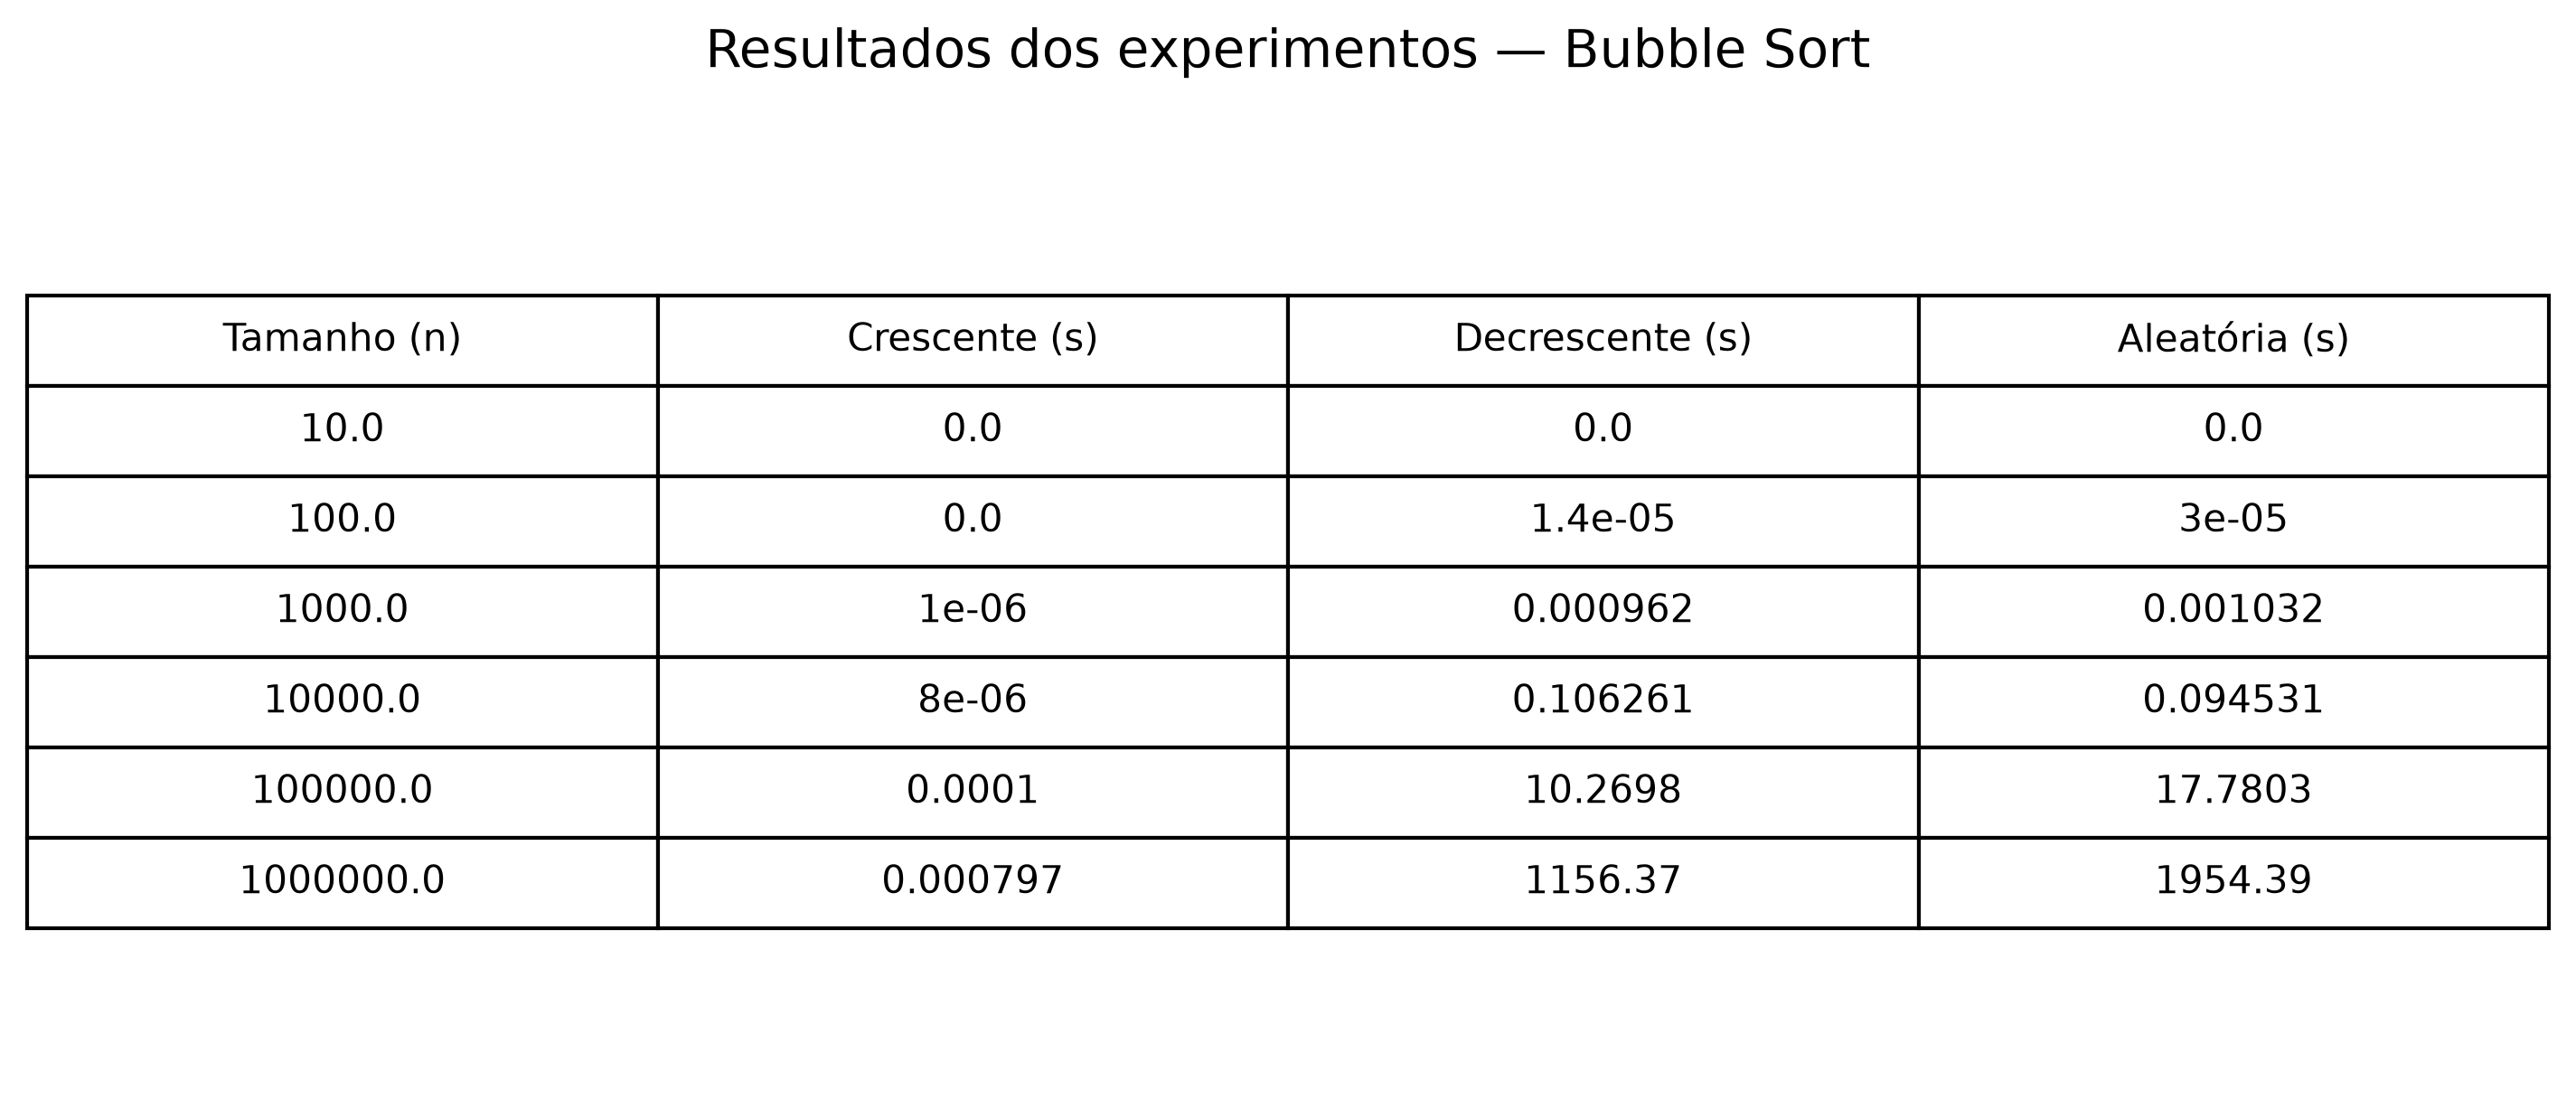
\includegraphics[width=16cm]{Imagens/Bubble_Sort/tabela.png}
\caption{Tabela de tempo de execução do algoritmo Bubble Sort}
\label{fig:tabela-bubble}
\end{figure}

\begin{figure}[H]
\centering
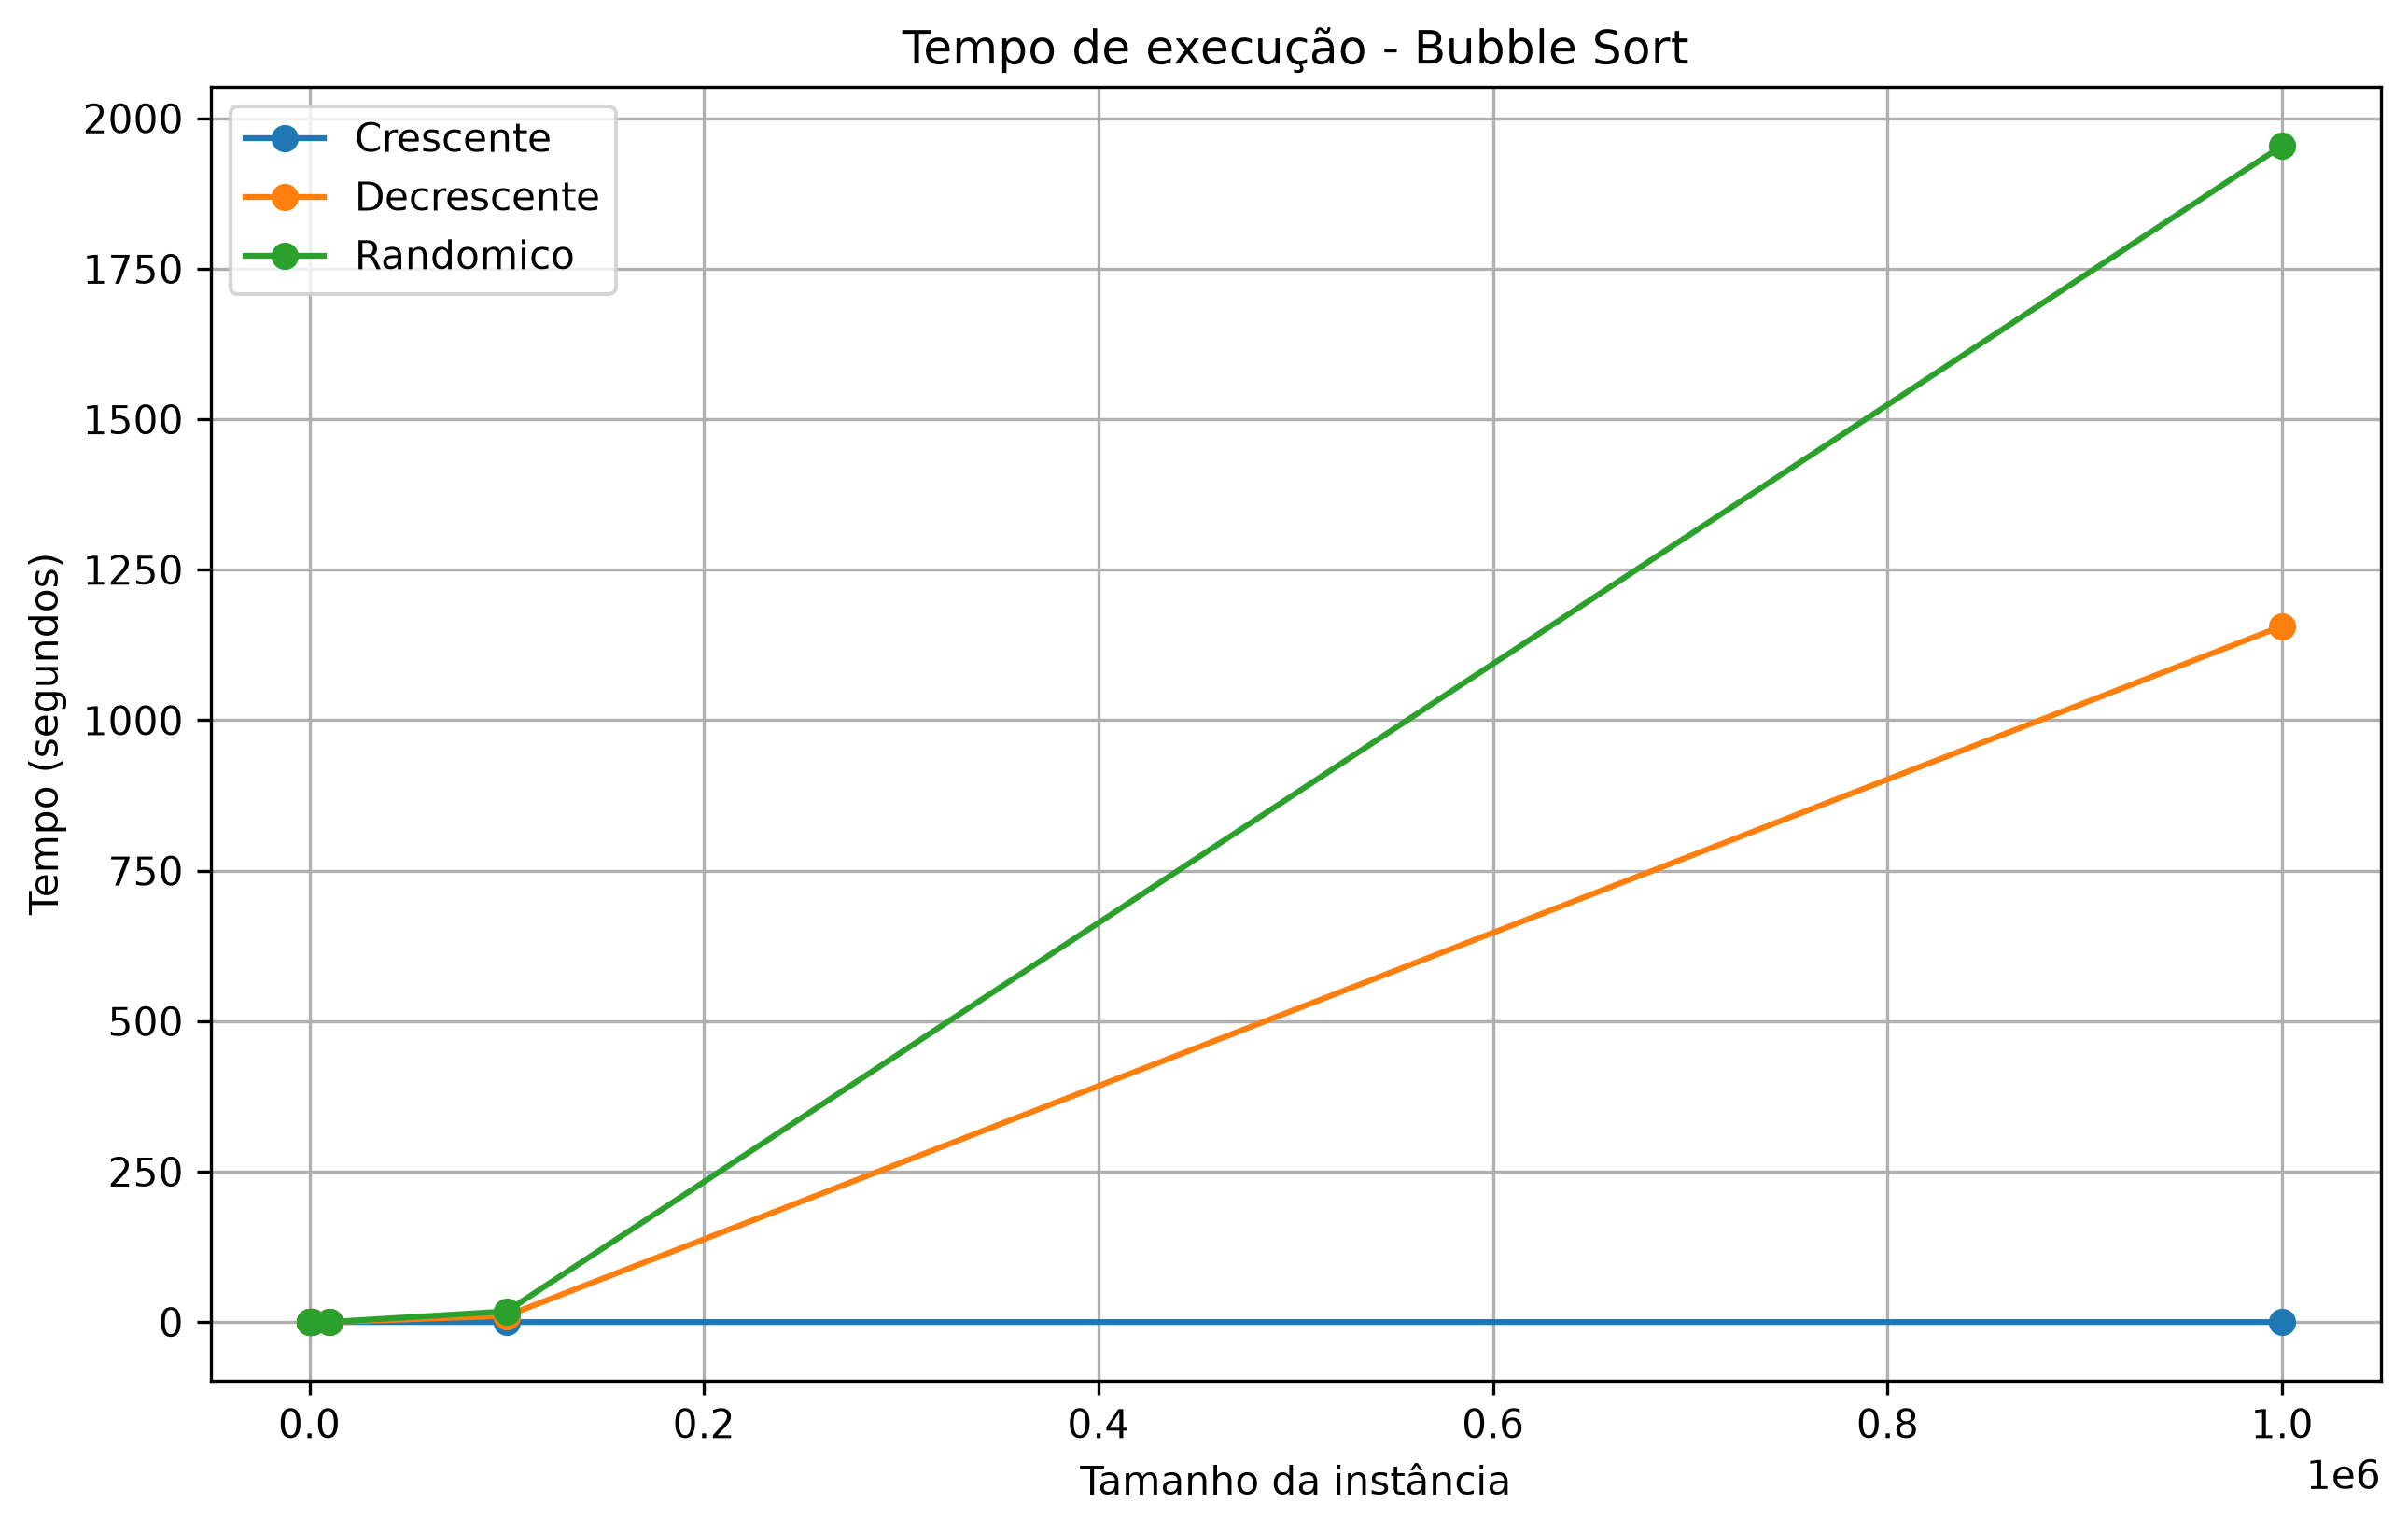
\includegraphics[width=10cm]{Imagens/Bubble_Sort/grafico.png}
\caption{Gráfico de tempo de execução do algoritmo Bubble Sort}
\label{fig:grafico-bubble}
\end{figure}

Os resultados obtidos nos experimentos estão apresentados na tabela e no
gráfico. Observa-se que o algoritmo Bubble Sort apresenta comportamentos
diferentes de acordo com a organização inicial dos elementos, devido à
utilização da variável \texttt{trocou}, que permite interromper a execução
quando nenhuma troca é realizada durante uma passagem.

Nas instâncias ordenadas de forma crescente, nenhuma troca é realizada
durante a primeira passagem. Dessa forma, a variável \texttt{trocou}
permanece com valor \texttt{false} e o algoritmo encerra sua execução por
meio do comando \texttt{break}, fazendo com que o melhor caso apresente
complexidade $\Theta(n)$.

Nas instâncias ordenadas de forma decrescente, além das comparações,
também são necessárias diversas trocas para colocar os elementos em suas
posições corretas. Como ocorre pelo menos uma troca durante cada passagem,
o comando \texttt{break} não é executado antes do término das passagens
previstas, caracterizando o pior caso do algoritmo, cuja complexidade é
$\Theta(n^2)$.

As instâncias aleatórias apresentam uma quantidade intermediária de
trocas, pois o número de elementos que precisam ser deslocados depende da
organização inicial do vetor. Entretanto, o algoritmo normalmente realiza
diversas passagens pelo vetor, fazendo com que o caso médio apresente
complexidade $\Theta(n^2)$.

A partir dos dados, também é possível perceber que o aumento do tamanho
da entrada provoca um crescimento significativo no tempo de execução,
principalmente nas entradas aleatórias e decrescentes. Nas entradas
crescentes, o algoritmo pode encerrar a execução após a primeira passagem,
devido à ausência de trocas.

Esses resultados apresentam comportamento compatível com a análise de
complexidade do algoritmo Bubble Sort, considerando a otimização utilizada
na implementação por meio da variável \texttt{trocou}.
